\section{SRAD Flight Computer Software Architecture}
\label{sec:Programming of the SRAD Computer}

An STM32 microcontroller was selected as the primary flight computer for the SRAD avionics system due to its high reliability, deterministic execution behaviour, and compatibility with the existing commercial off-the-shelf (COTS) avionics used by the team. These characteristics make the STM32 platform particularly well suited for safety-critical aerospace applications, where predictable operation and robust system performance are essential.

A major advantage of the STM32 architecture is its deterministic execution model. Unlike systems that rely on a general-purpose operating system, the STM32 executes firmware either in a bare-metal environment or under a lightweight real-time operating system (RTOS). This eliminates the unpredictability associated with background processes and non-deterministic task scheduling, ensuring that timing-critical operations are executed with consistent latency and repeatable behaviour. Functions such as sensor acquisition, telemetry transmission, state estimation, and recovery system control therefore operate within well-defined timing constraints. This deterministic behaviour significantly improves software validation and testing, which is essential for mission-critical systems.

The STM32 platform also provides hardware commonality with the team’s COTS avionics system, which operates as a redundant backup flight computer. Both systems are based on the same STM32 microcontroller family, allowing the same firmware codebase to be deployed across both platforms with minimal modification. This reduces software development complexity, minimises the risk of software divergence between systems, and simplifies debugging, testing, and long-term maintenance.

Firmware development is carried out using \textbf{STM32CubeIDE}, the official integrated development environment provided by STMicroelectronics. STM32CubeIDE was selected due to its integrated peripheral configuration tools, native STM32 support, hardware abstraction libraries, and advanced debugging capabilities. Using the official development ecosystem improves maintainability, ensures accurate peripheral configuration, and provides reliable debugging support during both development and ground testing.

The firmware architecture is implemented using \textbf{FreeRTOS}, enabling deterministic real-time task scheduling and modular software organisation. Critical subsystems operate concurrently as independent real-time tasks while maintaining predictable execution timing. Separate tasks are allocated for sensor acquisition, telemetry handling, flight-state management, data logging, and recovery system logic, improving scalability, software maintainability, and overall system reliability.

Communication between the SRAD flight computer and external systems is currently implemented using \textbf{UART} communication via the RX/TX interface. UART is used for telemetry transmission, debugging, and inter-device communication during development and testing.

Programming and debugging are performed using the \textbf{ST-LINK V2} interface, shown in Fig.~\ref{fig:USB_coms}. The ST-LINK V2 provides a stable interface between the development workstation and the STM32 microcontroller, enabling firmware uploading, real-time debugging, memory inspection, and breakpoint analysis.

\begin{figure}[H]
    \centering
    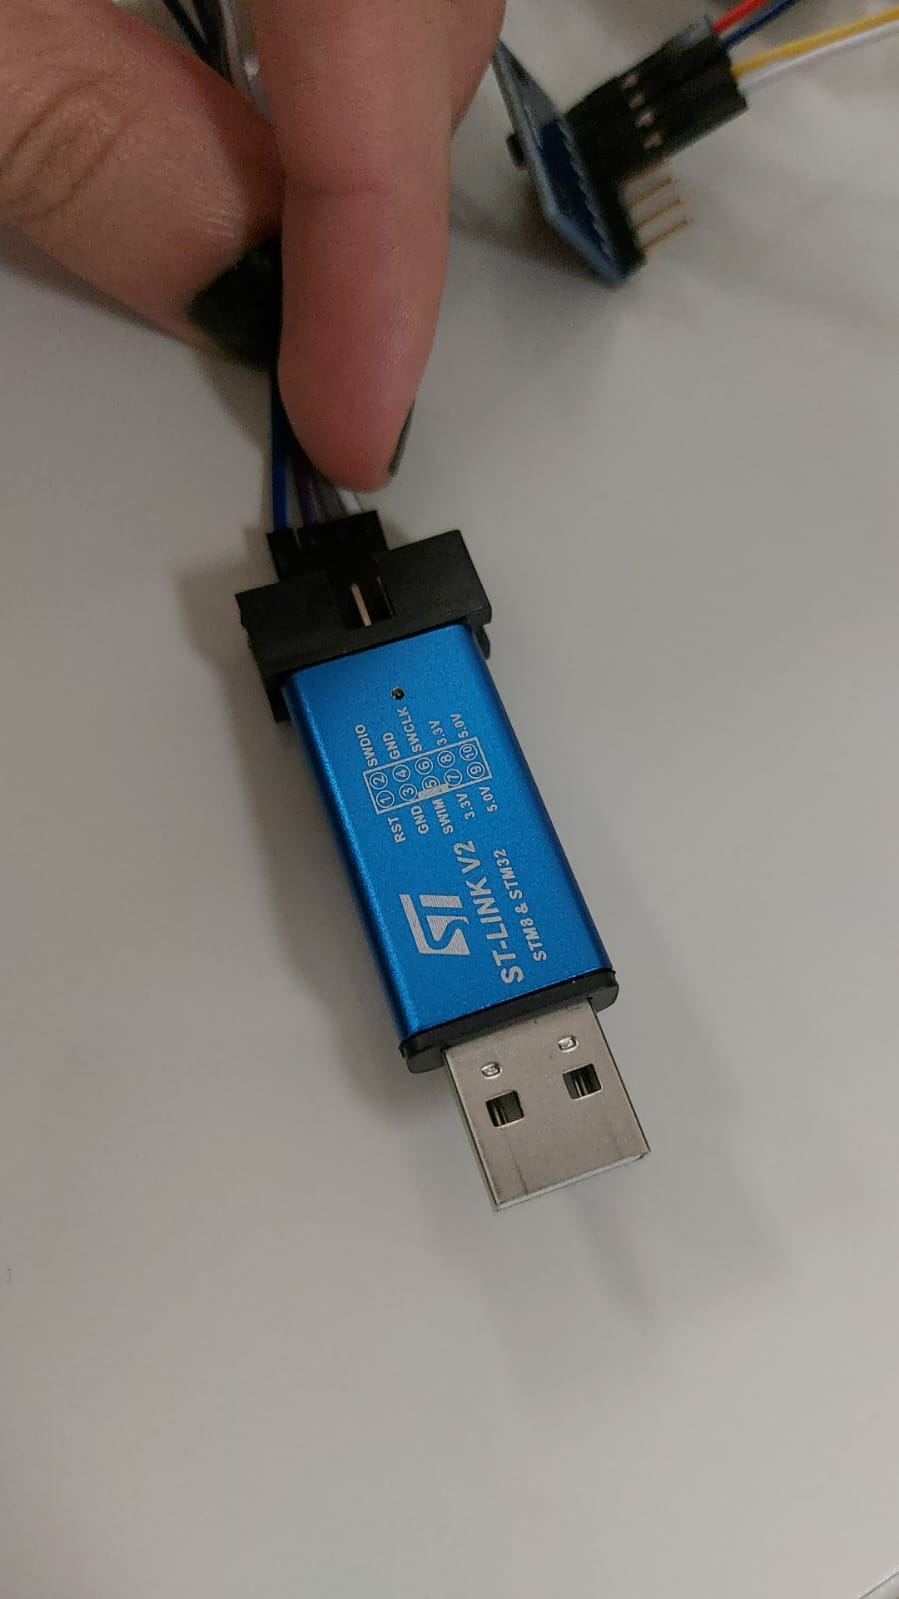
\includegraphics[width=\linewidth]{Images/3_Microcontroller/USB_coms.jpeg}
    \caption{ST-LINK V2 programmer/debugger interface}
    \label{fig:USB_coms}
\end{figure}

The complete hardware setup used during firmware development and testing is shown in Fig.~\ref{fig:current_setup}.

\begin{figure}[H]
    \centering
    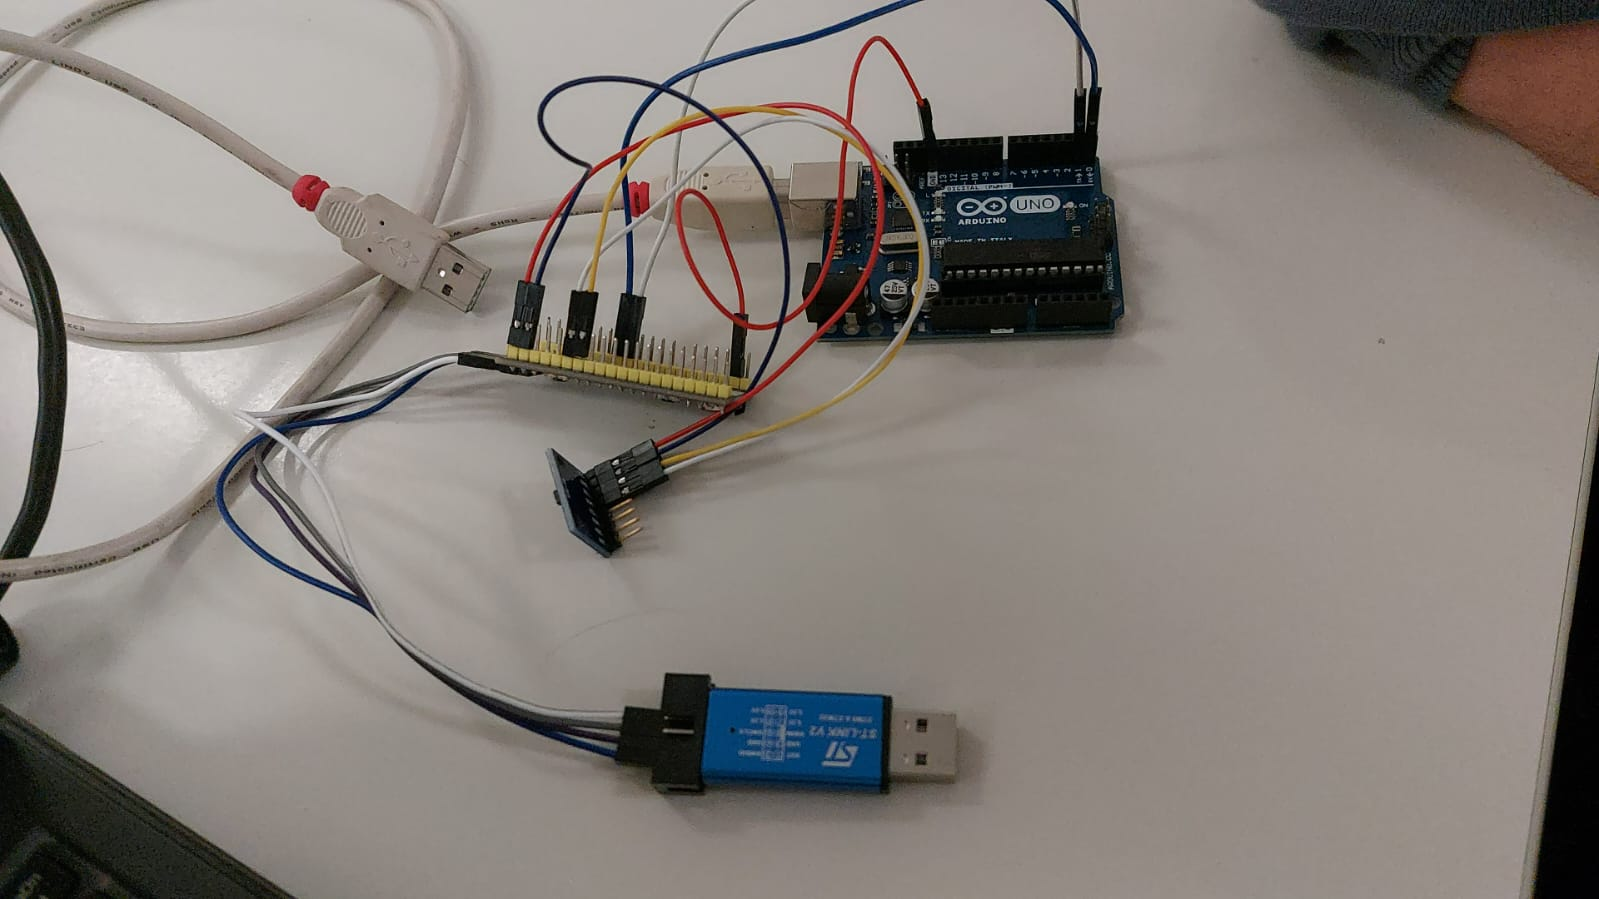
\includegraphics[width=\linewidth]{Images/3_Microcontroller/current_setup.jpeg}
    \caption{Current SRAD computer development setup}
    \label{fig:current_setup}
\end{figure}

The STM32F411 development board used for firmware implementation is shown in Fig.~\ref{fig:STM32411}.

\begin{figure}[H]
    \centering
    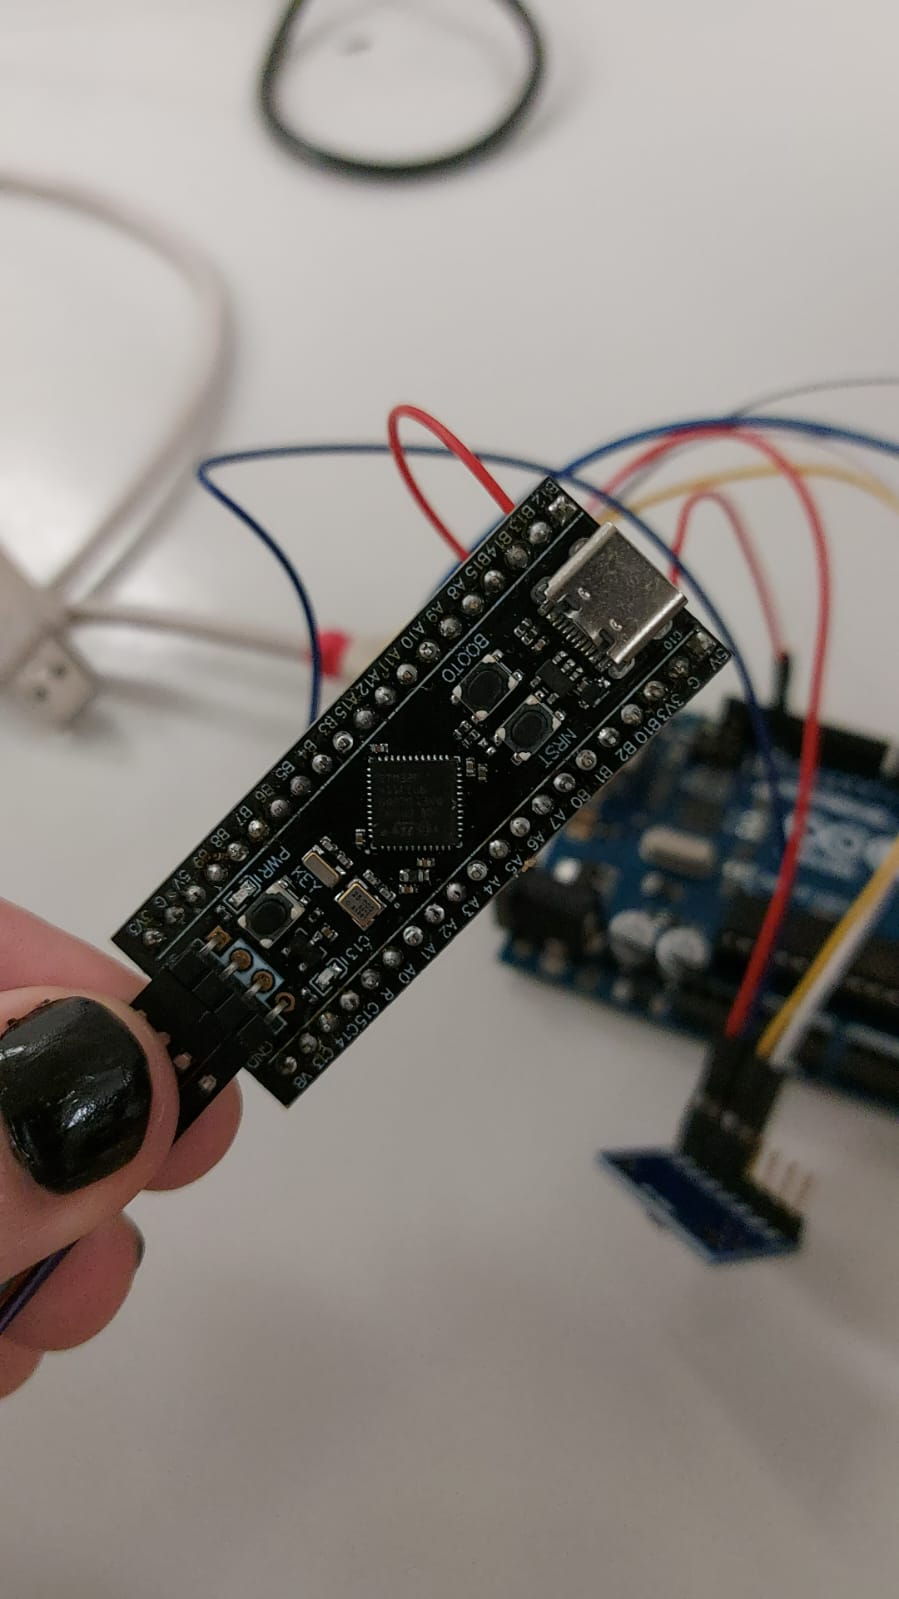
\includegraphics[width=\linewidth]{Images/3_Microcontroller/STM32411.jpeg}
    \caption{STM32F411 development board}
    \label{fig:STM32411}
\end{figure}

For initial communication testing and telemetry verification, UART communication was established between the STM32 and an Arduino Uno development board. In this configuration, inertial measurement unit (IMU) data is transmitted from the STM32 over the UART interface and monitored using the Arduino IDE serial monitor on a ground station computer. This arrangement provides a simple and effective platform for validating serial communication reliability and sensor data transmission prior to integration with the complete avionics stack.

The overall flight architecture incorporates both the SRAD flight computer and the COTS recovery system operating in parallel to provide redundancy and increased operational safety. The COTS recovery system is configured as the primary authority for parachute deployment and will always issue the recovery command when deployment conditions are satisfied. In the event of conflicting commands, the COTS system overrides the SRAD deployment signal. This hierarchical recovery structure introduces an additional safety layer and reduces the likelihood of deployment failure resulting from software or hardware anomalies within the SRAD system.

\subsection{Microelectronics}

\subsubsection{SRAD Electronics}

A summary of the primary electronic components used within the SRAD avionics system is provided in Anne, Table~\ref{tab:SRAD_electronics}. The table includes operating voltage ranges, typical current consumption, and estimated power usage where available.

\subsubsection{COTS Recovery Electronics}

The commercial off-the-shelf (COTS) recovery avionics system used as a redundant backup is also detailed in Annex, Table~\ref{tab:COTS_electronics}, including its supply requirements and power consumption.

\subsection{FreeRTOS}
\subsubsection{\texttt{task\_data\_acquisition}}

\textbf{Priority:} Very High

\textbf{Description:} This task is responsible for continuously reading raw data from the onboard sensors (Barometer, IMU, and GPS) at a strict and fixed frequency (e.g., 100\,Hz or 400\,Hz). By utilizing the \texttt{vTaskDelayUntil} function, it guarantees absolute timing execution without drift. To maintain its high-frequency execution rate and prevent blocking, this task intentionally avoids any complex calculations or data filtering. Its sole responsibility is to efficiently poll the I2C and SPI buses and immediately dispatch the gathered raw data to the relevant queues for downstream processing.

\subsubsection{\texttt{task\_filter}}

\textbf{Priority:} High

\textbf{Description:} This task receives the raw data from the sensors and processes it through Kalman filter. Its primary objective is to take noisy sensor readings and calculate clean, accurate estimates for true altitude, velocity, and acceleration. These are the exact state variables required by the flight control state machine to safely and accurately trigger phase transitions.




\subsection{Electronics Bay Configuration}

The avionics bay provides the internal working volume required to house the SRAD and COTS electronics systems. The available internal dimensions are listed below:

\begin{itemize}
    \item \textbf{Length:} 300\,mm
    \item \textbf{Inner Diameter:} 119\,mm
\end{itemize}

The planned PCB arrangement within the avionics bay is illustrated in Fig.~\ref{fig:PCB_diag}.

\begin{figure}[H]
    \centering
    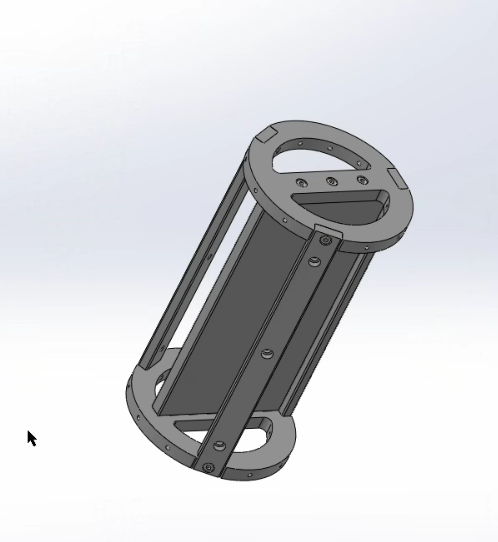
\includegraphics[width=0.85\linewidth]{Images/2_eletronic_components/PCB_diag.png}
    \caption{Planned PCB placement inside the avionics bay}
    \label{fig:PCB_diag}
\end{figure}

Table~\ref{tab:PCB_designations} identifies the function of each PCB within the avionics stack.

\begin{table}[H]
\centering
\caption{PCB functional designations}
\label{tab:PCB_designations}
\begin{tabular}{ll}
\toprule
\textbf{PCB} & \textbf{Designation} \\
\midrule
PCB 1 & SRAD Electronics \\
PCB 2 & COTS Electronics \\
PCB 3 & Power Supply Unit (PSU) \\
\bottomrule
\end{tabular}
\end{table}